\documentclass[12pt,onecolumn]{article}
\usepackage{epsfig}
\usepackage{natbib}
\usepackage{caption}
\usepackage{multicol,wrapfig}
%\usepackage{deluxetable}
\usepackage{graphics,graphicx}
\usepackage{rotating}
\usepackage{amssymb}
\usepackage{amsmath,fancyhdr}
%\usepackage{tweaklist}
\usepackage{cuted}
\usepackage{hyperref}
\usepackage{xspace}
\usepackage[table]{xcolor}
\usepackage{listings}

\definecolor{codegreen}{rgb}{0,0.6,0}
\definecolor{codegray}{rgb}{0.5,0.5,0.5}
\definecolor{codepurple}{rgb}{0.58,0,0.82}
\definecolor{backcolour}{rgb}{0.95,0.95,0.92}

% Add space between paragraphs
\setlength{\parskip}{0.4\baselineskip}%
% Add or remove space between lines (1.0 = default spacing)
\linespread{1.0}
\setlength{\parindent}{0pt} % no paragraph indent

\citestyle{abbrv}

%\citestyle{aa}
%\citestyle{nature}
%\bibpunct[,]{[}{]}{,}{n}{,}{}

%\renewcommand{\rmdefault}{cmr}

%\newcommand{\phil}[1]{ \textcolor{blue}{\bf #1} }

\makeatletter
\renewcommand{\section}{\@startsection%
{section}{1}{0mm}{-0.5\baselineskip}%
{0.1\baselineskip}{\large\normalfont\bfseries}}%
\renewcommand{\subsection}{\@startsection%
{subsection}{1}{0mm}{-0.2\baselineskip}%
{0.1\baselineskip}{\normalfont\bfseries}}%
\makeatother

\setlength{\textwidth}{6.5in}
\setlength{\textheight}{9in}
\setlength{\topmargin}{0in}
\setlength{\oddsidemargin}{0in}
\setlength{\evensidemargin}{0in}
\setlength{\headheight}{0in}
\setlength{\headsep}{0in}
\setlength{\hoffset}{0in}
\setlength{\voffset}{0in}
\setlength{\textfloatsep}{0.0in}
\setlength{\floatsep}{0.0in}

\lstdefinestyle{mystyle}{
    backgroundcolor=\color{backcolour},   
    commentstyle=\color{codegreen},
    keywordstyle=\color{magenta},
    numberstyle=\tiny\color{codegray},
    stringstyle=\color{codepurple},
    basicstyle=\ttfamily\footnotesize,
    breakatwhitespace=false,         
    breaklines=true,                 
    captionpos=b,                    
    keepspaces=true,                 
    numbers=left,                    
    numbersep=5pt,                  
    showspaces=false,                
    showstringspaces=false,
    showtabs=false,                  
    tabsize=2
}

\lstset{style=mystyle}

\newcommand{\be}{\begin{eqnarray}}
\newcommand{\ee}{\end{eqnarray}}
\newcommand{\code}[1]{\lstinputlisting[language=Python]{#1}}
\renewcommand{\theequation}{\thesection.\arabic{equation}}
\numberwithin{equation}{section}
\renewcommand{\vec}[1]{\boldsymbol{#1}}
\newcommand{\mtx}[1]{\boldsymbol{#1}}
\newcommand{\grad}{\vec{\nabla}}
\newcommand{\order}{\mathcal{O}}

\newcommand{\dddt}[1]{\frac{\partial^2 #1}{\partial t^2}}
\newcommand{\dddx}[1]{\frac{\partial^2 #1}{\partial x^2}}
\newcommand{\ddt}[1]{\frac{\partial #1}{\partial t}}
\newcommand{\ddx}[1]{\frac{\partial #1}{\partial x}}
\newcommand{\gradd}{\nabla^2}
\newcommand{\vel}{\vec{v}}
\newcommand{\Fourier}[1]{\mathcal{F}(#1)}

\begin{document}
{\large \bf Brief Primer on Statistical and Numerical Methods in Python}

%\input{data.tex}
\section{Ordinary Differential Equations}

\subsection{Euler's Method}

Consider the following first order ordinary differential equation.
\be
\frac {d\vec{y}}{dt} = \vec{f}(\vec{y}, t),
\ee
where $\vec{y}$ is a vector of variables, $t$ is the independent variable, and $\vec{f}$ is some arbitrary vector function of $\vec{y}$ and $t$.  We can use our definition of derivative to write: 
\be
\frac {d\vec{y}}{dt} \approx \frac {\vec{y}_{i+1} - \vec{y}_i}{\Delta t} = \vec{f}(\vec{y}_i, t_i),\label{eq:explicit}
\ee
where $\Delta t = t_{i+1} - t_i$.  This is not the only choice that could have been made, it is also possible to write it as 
\be
\frac {\vec{y}_{i+1} - \vec{y}_i}{\Delta t} = \vec{f}(\vec{y}_{i+1}, t_{i+1}). \label{eq:implicit}
\ee
The difference between these two is the choice of either $t_{i}$ or $t_{i+1}$ on the right hand side.  Equation (\ref{eq:implicit}) gives rise to implicit methods which are harder to code up, but offers potentially greater stability and speed.  Instead, we will focus on equation (\ref{eq:explicit}).  

If we know the value at $\vec{y}(t_i)$, we can solve for $\vec{y}(t_{i+1})$ to be
\be
\vec{y}_{i+1} = \vec{y}_i + \vec{f}(\vec{y}_i, t_i)\Delta t.\label{eq:euler method}
\ee
This method is known as Euler's method.  As an aside, it we take $\vec{f}$ to be a scalar function of just $t$, then it just becomes an ordinary integral.  Hence, the methodology we describe here is directly relevant for numerical integration so we don't need a separate discussion for it.

Equation (\ref{eq:euler method}) gives the correct answer for $\Delta t \rightarrow 0$, but it should never be used solving any equations you code up on a computer as superior methods abound. But it is easy and simple to code up and introduces the idea of generic algorithms.  

\subsection{Second Order Runge-Kutta Method}

Runge-Kutta methods are an example of predictor-corrector methods.  That is, it ``predicts'' the value at $\vec{y}_{i+1}$ from the current solution at $\vec{y}_i$.  Using this predicted value, it performs a ``corrector'' step to increase the accuracy of the solution.  The generic two-step Runge-Kutta method is as follows:
\be
\vec{k}_1 &=& \Delta t \vec{f}(\vec{y}_i, t_i) \\
\vec{k}_2 &=& \Delta t \vec{f}(\vec{y}_i + \beta \vec{k}_1, t_i + \alpha \Delta t) \\
\vec{y}_{i+1} &=& \vec{y}_i + a \vec{k}_1 + b \vec{k}_2
\ee
where $\vec{k}_1$ is the ``predictor'' and is the same as an Euler step, $\vec{k}_2$ is the ``corrector'', and the $i+1$ step is some linear combination of the two.  The constants, $\alpha$, $\beta$, $a$, and $b$ are chosen to make the entire algoritm accurate to $\mathcal{O}(\Delta t^3)$.  To determine these unknown constants, let perform a Taylor expansion of $\vec{y}_{i+1}$
\be
\vec{y}_{i+1} = \vec{y}_i + \frac{d\vec{y}}{d t}(t_i)\Delta t + \frac 1 2 \frac{d^2\vec{y}}{dt^2}(t_i)\Delta t^2
\ee
Now 
\be
\frac{d^2\vec{y}}{dt^2}(t_i) &=& \frac {d\vec{f}(\vec{y},t)}{dt} = \frac {\partial \vec{f}(\vec{y},t)}{\partial t} + \frac{d\vec{y}}{dt}\cdot\vec{\nabla}_{\vec{y}}\vec{f} \\
&=& \frac {\partial \vec{f}(\vec{y},t)}{\partial t} + \vec{f}\cdot\vec{\nabla}_{\vec{y}}\vec{f}
\ee  
Thus we have 
\be
\vec{y}_{i+1} = \vec{y}_i + \vec{f}(\vec{y}_i, t_i)\Delta t + \frac 1 2 \left(\frac {\partial \vec{f}(\vec{y}_i,t_i)}{\partial t} + \vec{f}(\vec{y}_i,t_i)\cdot\vec{\nabla}_{\vec{y}}\vec{f}(\vec{y}_i,t_i)\right)\Delta t^2 +\mathcal{O}(\Delta t^3)\label{eq:2nd order}
\ee
Now we Taylor expand out $\vec{k}_2$ to find
\be
\vec{k}_2 &=& \Delta t \vec{f}(\vec{y}_i + \beta \vec{k}_1, t_i + \alpha \Delta t) \\
&=& \Delta t\left( \vec{f}(\vec{y}_i, t_i) + \alpha\Delta t\frac {\partial \vec{f}(\vec{y}_i,t_i)}{\partial t} + \beta\Delta t \vec{f}\cdot\vec{\nabla}_{\vec{y}}\vec{f}(\vec{y}_i,t_i)\right)
\ee
Putting this all together, we have 
\be
\vec{y}_{i+1} &=& \vec{y}_i + (a+b)\Delta t \vec{f}(\vec{y}_i, t_i) + b\Delta t^2\left(\alpha\frac {\partial \vec{f}(\vec{y}_i,t_i)}{\partial t} + \beta\vec{f}\cdot\vec{\nabla}_{\vec{y}}\vec{f}(\vec{y}_i,t_i) \right)+\mathcal{O}(\Delta t^3)\label{eq:rk2 expansion}
\ee
Comparing Equations (\ref{eq:2nd order}) and (\ref{eq:rk2 expansion}), we get the following conditions:
\be
a+b = 1 \qquad b\alpha = \frac 1 2 \qquad b\beta = \frac 1 2,
\ee
or 3 equation for 4 unknowns.  So that mean there exist a infinite number of second order schemes that are possible, e.g., error per step that goes likes $\Delta t^3$, so the total error over an interval goes like $\Delta t^2$.  So using $\alpha$ as a parameter, we have 
\be
\beta = \alpha \qquad b = \frac 1 {2\alpha} \qquad a = 1 - \frac 1 {2\alpha}
\ee
So a generic second order Runge-Kutta scheme is then
\be
\vec{k}_1 &=& \Delta t \vec{f}(\vec{y}_i, t_i) \\
\vec{k}_2 &=& \Delta t \vec{f}(\vec{y}_i + \alpha \vec{k}_1, t_i + \alpha \Delta t) \\
\vec{y}_{i+1} &=& \vec{y}_i + \left(1 - \frac 1 {2\alpha}\right) \vec{k}_1 + \frac {\vec{k}_2} {2\alpha} 
\ee

A few famous examples are 
\begin{itemize}
    \item Midpoint method: $\alpha = 1/2$ Estimate the values of y at the midpoint and solve for the derivative at the midpoint.  Use this midpoint derivative to complete the integration.  Note that prefactor in front of $\vec{k}_1$ in this case is zero.
    \item Heun's Method: $\alpha = 1$ Estimate the values of y at the endpoint and give equal weight to both starting and endpoints to compute the derivative.
\end{itemize}

It turns out that for the most part this is all you really need.  We should use the generic ode solvers that come with scipy generally. 

\subsection{Higher Order ODEs}

Thus far we have discussed the case of first order odes.  What about higher order ODEs.  It turns out that there is a very simple extension to arbitrary high order ODEs.  The trick is it identify higher order derivatives as variables in themselves.  Consider the ODE
\be
\sum_n^N\frac{d^n f}{dx^n} = 0
\ee
We can write this as a sum first order ODEs by the identification of 
\be
f_i = \frac{df_{i-1}}{dx} \qquad\textrm{and}\qquad f_0 = f
\ee
Thus we have 
\be
\frac{df_{N-1}}{dx} + \sum_i^{N-1} f_i = 0,\\
\frac{df}{dx} = f_1\\
\frac{df_1}{dx} = f_2\\
 . . . . \\
\frac{df_{N-2}} = f_{N-1}.
\ee
So this converts a Nth order ODE to N first order ODEs, which we can solve.

\subsection{Timestepping}

One thing that we have not discussed is the choice for $\Delta t$.  For an interval between $t_0$ and $t_1$, a larger $\Delta t$ results in fewer computational steps, which makes things faster.  However, a smaller $\Delta t$ results in greater accuracy.  There is a limit with higher order methods on how accurate you can make a solution.  

But there is another subtle issue that can happen.  In many instances the right hand side of an ODE can take on large (positive or negative) values for a limited set of circumstances.  In these cases, it is useful to have a variable $\Delta t$ -- small when things change quickly and large when things change slowly.  How can we estimate when these occurs.  

Suppose you have an ODE of the form
\be
\frac{\partial y}{\partial t} = f(y,t)
\ee
Then according to Euler's method we have
\be
y_{n+1} - y_n = f(y_n,t_n)\Delta t
\ee
Now suppose we want the change in $\Delta y = |y_{n+1} - y_n| < \alpha |y_n|$.  This means that
\be
\alpha |y_n| = |f(y_n,t_n)|\Delta t_{\rm max}
\ee
This allows us to solve for $\Delta t_{\rm max}$ to be
\be
\Delta t_{\rm max} = \alpha \left|\frac{y_n}{f(y_n,t_n)}\right|
\ee
Typically, you don't want $\alpha$ to be too large nor too small.  I have found values between 0.01 and 0.1 to work well.  

At the same time, we don't want to miss something if $\Delta t_{\rm max}$ is too large that it totally misses a change.  In this case, I like to pick a $\Delta t_{\rm max,0} = (t_1 - t_0)/N_0$, where $N_0$ is a number between 10 or 100, but this can change as well.

So a selection for $\Delta t$ at a time $t$ would be
\be
\Delta t = min( t_1 - t, min(\Delta t_{\rm max,0}, \Delta t_{\rm max}))
\ee

Now lets try an example of this.
\newpage
\section{Optimization and Parallelization}

\subsection{Optimization}

There are two kinds of optimization.  There is optimizing human time and effort and optimizing machine time and effort.  Generally human time and effort is far more valuable than machine time and effort which is why we have use python in this class even though it is thousands of times slower than C or fortran.  The reason is that it is far cleaner and easier to use and link up to libraries than C or fortran.  

However, this is not always the case and so we should discuss a few ways to do optimization and parallelization of code. In this section we will discuss python optimization.  The key fact about python optimization is several-fold.  But before optimizing you should consider the following questions
\begin{enumerate}
    \item Is your code correct?
    \item Do you need to optimize?
    \item Do you really need to optimize?
    \item Optimize is not parallelization -- usually do this last.
    \item Optimization involves tradeoffs.  Be careful what you wish for.
\end{enumerate}

There are a few steps to optimization:
\begin{enumerate}
\item profile
\item profile again.
\item check the hotspots.
\item payoff in optimization: modify your use case, use better algorithms, use builtin functions, use numba, pre-compiled code
\end{enumerate}

So at this point, you have decide to optimize.  We will take the N-body problem we discussed earlier as a starting point. Jupyter notebooks has a really useful magic function for profiling called \%prun.  Lets see this in action.

\textbf{Go to Jupyter notebook.}

Now we will optimize this function in several ways.  These are in order:
\begin{enumerate}
    \item Writing optimal python -- using numpy functions whenever possible -- for this case I got a speedup of 4-5x
    \item Using Numba -- this works well with numpy code.  It use a decorator @jit or @njit which using a just-in-time compiler for great speedups.  This is super easy, but also you have no control over what it does, so the result can be good or horrible.  
    \item Using cython -- this requires some knowledge of c and data types that is native to computers.
    \item Using fortran and f2py -- I got a 600x speedup with this. 
\end{enumerate}

For fortran and cython, it is important to keep in mind that c and to some extent fortran has been the dominant language/scheme of computing over the last 50 years and so to some degree processors are designed to work with these languages. At one point, there was designs to build cpus optimized for lisp (scary thought).  Let think about how a cpu works.  

A cpu consists of a integer unit and a floating point unit.  Early cpus prior to the pentium are mostly an integer unit and floating point was slow.  But these days integer and floating point computations are similarly fast.  So the native data types that give great speed are int and float (or double).  So you want to map it to these things whenever you can. 

So the key idea for cython is to take your python code and judiously use ``cdef int'', ``cdef double'', or ``cdef double []'' in the correct places to greatly speed up the code.  

\subsection{Parallelization}

The choice of python for this course was unfortunate in one crucial aspect and that is the ability of python to be parallelized easily on one machine.  Modern cpus have $>4$ cores and thus the ability to use more than one core for computation are a real boon.  Python is especially limited in this respect, but there are parallelization methods that we can discuss for python.  

The simpliest parallelization strategy that you will encounter and probably the most common is ``embarassingly'' parallel.  This occurs is many situations such as large data analysis or parameter studies.  Generally the paradigm that one should think about for ``embarassingly'' parallel problems is something called MapReduce.  Here we map a computation to a large number of computers/cores and then reduce the information to a simpler data set at the end.  To see how this works, let us consider the counting of the numbers of words in ``War and Peace''.  You could do this by sitting down and counting the entire book, or you can assign each page to a different person.  Each person will count the words on the page and you can just add up all the counts together.  The assignment of a person to a task is the map and the collation of information returned is the reduce part.  

There are several ways of doing map-reduce.  Here are a few off the top of my head:
\begin{itemize}
    \item shell-script
    \item gnu-parallel
    \item python multiprocessing pool
    \item python MPI
    \item condor/open science grid
\end{itemize}

Lets discuss a few in turn.  

Here is a example shell script
\begin{lstlisting}[language=bash]
#!/bin/bash

do-job-1 &
do-job-2 &
wait
\end{lstlisting}
Pretty simple.  We do 2 jobs and we wait until it is finish.  Very simple, but it can be tedious to code especially for large number of jobs.

Here is an example for gnu-parallel
\begin{lstlisting}[language=bash]
#!/bin/bash

seq 1 1 100 | parallel -j 8 python job-name {}

\end{lstlisting}
seq counts from 1 to 100 in steps of 1 and parallel execute up to 8 jobs at once wher the label in \{\} is the number labeled by seq.  Great way to doing an arbitrary number of jobs on a cluster.  gnu-parallel is usually used on one node, but multiple  nodes can use used if you know how. 

There are a few ways of doing multiprocessing on python -- having a single python instance launch multiple instances and run different things on them.  Here I will introduce multiprocessing pools as I have experience with them.  Ideally, you should use python executors as this much more future proof, but the future proof part is fairly far away. 
\begin{lstlisting}[language=Python]
def func( x) : 
    print(x)

import multiprocessing as mp
with mp.Pool(processes=4) as pool :
    result = pool.map(func, np.arange(100))
\end{lstlisting}
This is awesome, map and reduce in essentially one one.  It returns the result as a list in the same order of the original map and thus is can be reduces as soon as one prefers.  

Finally lets talk a bit about mpi.  The structure of MPI is as follows.  At startup N programs launch and are able to communicate with each other.  On startup you will get a comm object,
\begin{lstlisting}[language=Python]
from mpi4py import MPI

comm = MPI.COMM_WORLD
rank = comm.Get_rank()
\end{lstlisting}
The rank is the identifier of your process.  rank==0 is the first program and usually acts as an overseer for everything else.  So for instance suppose you want to do a map reduce in MPI. 
\begin{lstlisting}[language=Python]

if rank == 0:
    data = [(i+1)**2 for i in range(size)]
else:
    data = None
data = comm.scatter(data, root=0)
\end{lstlisting}
Here comm.scatter recognized that the data that is to be mapped comes from the rank == 0 process.  All other processes (including root) will then get a subset of data to play with.  To reduce, we must do a gather
\begin{lstlisting}[language=Python]
    data = comm.gather(data, root=0)
    if rank == 0:
        # do something with the data
        pass
\end{lstlisting}
    
%\newpage 
%\section{Partial Differential Equations}

Partial Differential equations (PDEs) are the heart of many physical systems that we are interested in.  We will study three main classes of PDEs
\begin{enumerate}
    \item Hyperbolic
    \item Elliptic
    \item Parabolic
\end{enumerate}

\noindent\textbf{Hyperbolic:}
Hyperbolic PDEs characterized by real distinct propagation speeds.  As such their usual physical intepretation involves a state that evolves in time in accordance to a known signal speed. An example of this is the wave equation:
\be
\dddt{f} - \dddx{f} = 0
\ee
To solve these equations they require boundary conditions in space and initial conditions in time. The most typical example of hyperbolic equations are the compressible fluid equations.  

\noindent\textbf{Elliptic:}
Elliptic PDEs characterized by effectively infinite propagation speeds.  As such they require boundary conditions everywhere as their solution relies on the BCs.  Their solutions are also smooth.  An example of this is the Poisson equation:
\be
\dddt{f} + \dddx{f} = g
\ee
In addition to Poisson, other examples of elliptic equation are electrostatics, (Newtonian) gravity, etc.  Incompressible fluid flow also has an elliptic nature as the incomoressibility conditions is elliptic. 

\noindent\textbf{Parabolic:}
Parabolic PDEs somewhat between hyperbolic and elliptic equations. They do propagrate in time so only require boundary conditions on the spatial part and while they can allows sharp solutions, it likes to smooth it out.  An example is the diffusion equation"
\be
\ddt{f} - \dddx{f} = 0
\ee

The origin of the name comes from a classification of conic sections.  For instance for a general PDE:
\be
au_{xx} + bu_{xy} + cu_{yy} + du_x + e u_y + f = g
\ee
It is hyperbolic if $b^2 - 4ac > 0$, elliptic if $b^2 - 4ac < 0$ and parabolic if $b^2-4ac = 0$.  

Now we already know how to solve ODE problems so our goal here is to convert PDEs to ODEs and use the standard techniques to solve them.  There is no general way of converting an arbitrary PDEs to an ODE though this can be done for certain problems by defining a new variable that mixes two or more of the independent variables, e.g., self-similar methods.  However, this works for a very special subset of problems and don't work generally. 

As a result, the usual method for solving (hyperbolic and parabolic) PDEs is to descretized space and approximate the spatial derivatives on that space and use ODE solvers to advance the solution in time.  There are a number of possible ways to do this. 
\begin{enumerate}
    \item finite difference: values of a function are stored at discrete points -- replace derivatives with 
    \item finite volume: the values of a function are average over the volume centered around a grid point.  Because of this, the methods here involve replacing differentiation with integration of a flux over a the boundary of the volume.
    \item finite element: kinda like spectral methods, but with compact basis functions. 
    \item spectral methods: decompose the values of a function on space to Fourier components. Solve for the evolution of the Fourier components. Amazing for smooth flows - exponential convergence.
    \item particle methods: break up space into discrete sampled points the evolve at some velocity -- only really useful for hyperbolic equations.
\end{enumerate}

\subsection{Advection and Hyperbolic Problems}

We will begin first with the linear advection problem as many hyperbolic problems can be rewritten in a manner similar to advection. 
\be
\ddt{f(t,x)} + v\ddx{f(t,x)} = 0,
\ee
where $v$ is some propagating speed. We will assume some initial condition $f(0,x)$ and lets assume periodic boundary conditions $f(t,0) = f(t,L)$.  The solution to this problem is trivial: $f(t,x) = g(x-vt)$ for any arbitrary function $g$.  Because such a simple analytic solution exists, these is an ideal test case to test the error of whatever method we bring to bear.

\subsubsection{Finite Difference}

The first way we will look at this is via finite difference. Lets try a very simple discretization:
\be
\frac{f^{n+1}_i - f^n_i}{\Delta t} - v\frac{f^n_{i+1} - f^n_{i-1}}{2\Delta x} = 0
\ee
This is centered differencing in space and first order differencing in time or FTCS.  For a constant $v$, we can write this as
\be
f^{n+1}_i = f^n_i - \frac{v\Delta t}{2\Delta x}\left(f^n_{i+1} - f^n_{i-1}\right) = f^n_i - \frac{\alpha_{\rm CFL}}{2}\left(f^n_{i+1} - f^n_{i-1}\right),
\ee
where $\alpha_{\rm CFL} = v\Delta t/\Delta x$ is called the Courant-Friedrichs-Levy (CFL) number.  By setting this number, we force what $\Delta t$ will be.  This is the timestep. For stability, $\alpha_{\rm CFL} < 1$ and can be much smaller than unity. This is the same statement as information does not propagate more then one cell at a time.  

We write a simple code to evolve the advection equations here.  It evolves a simple gaussian or tophat profile across a period box of length $L=1$ at a velocity of $v=1$.  The CFL number is 0.8.  We will present the code later on, but the evolution part looks like this:

\begin{lstlisting}[language=Python]
def ftcs(f, dt, dx, cfl=cfl) :
    pass
\end{lstlisting}

If we evolve this, we see that the code appears stable for a little while before it falls apart.  For the tophat profile the situation is dire immediately.  

Now the issue is the FTCS is not stable and, in fact, it is what we call unconditionally unstable, which is a bad state of affairs.  The reason for this is that information in flows moves from upstream to downstream, but the ftcs scheme above allows information to flow from downstream to upstream.  So like the future affecting the past, this is now allowed and results in the destruction of the computational universe.  

To resolve this lets define two first order spatial derivatives
\be
\frac{f^{n+1}_i - f^n_i}{\Delta t} - v\frac{f^n_{i+1} - f^n_{i}}{\Delta x} = 0 \qquad\textrm{for\ } v < 0\\
\frac{f^{n+1}_i - f^n_i}{\Delta t} - v\frac{f^n_{i} - f^n_{i-1}}{\Delta x} = 0 \qquad\textrm{for\ } v > 0 
\ee
where we pick the upwind difference, e.g., we look at which way the flow is coming.  

Lets look at the complete code now.

\lstinputlisting[language=Python]{code/advection_ftcs.py}

There are other methods to do the solutions other than upwinding.  These include Lax-Friedrichs and Lax-Wendroff, but we will move onto finite volume methods.   

Before doing so, we should discuss convergence. Convergence is the measure of how accurately a numerical method reproduces the exact solution.  In the case of ODEs, we care about the accuracy of 
\be
{\rm Err} = 2\left|\frac{f_{\rm num}(t_{\rm end}) - f_{\rm analytic}(t_{\rm end})}{f_{\rm num}(t_{\rm end})+f_{\rm analytic}(t_{\rm end})}\right|
\ee
So the error is taken only at the end point.  For hyperbolic equations, we can think of this as a set of ODEs and so we the error is 
\be
{\rm Err} = 2N^{-1}\sum_i\left|\frac{f_{i,\rm num}(t_{\rm end}) - f_{i,\rm analytic}(t_{\rm end})}{f_{i, \rm num}(t_{\rm end})+f_{i,\rm analytic}(t_{\rm end})}\right|
\ee
This is actually called the L1 norm. Another version if the L2 norm, which is 
\be
{\rm Err} = 2\sqrt{N^{-1}\sum_i\left(\frac{f_{i,\rm num}(t_{\rm end}) - f_{i,\rm analytic}(t_{\rm end})}{f_{i, \rm num}(t_{\rm end})+f_{i,\rm analytic}(t_{\rm end})}\right)^2}
\ee
I don't have any advice on which one to choose, but for this version we will look at the L2 norm.  This gives a error as a function of N that goes $N^{-1}$
\begin{figure}
    \centering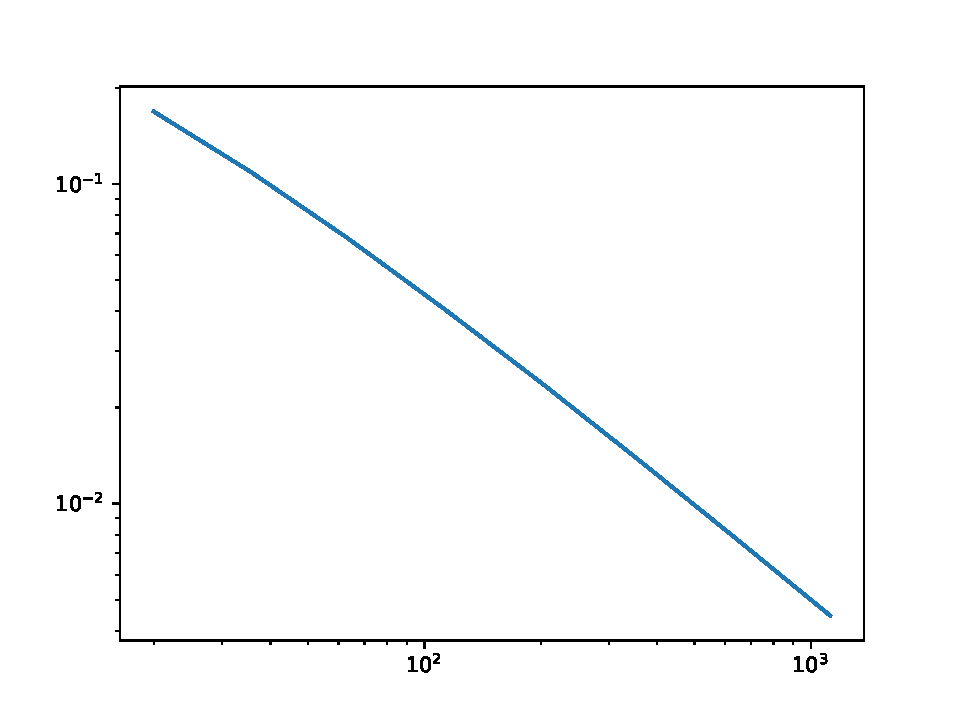
\includegraphics[width=0.75\textwidth]{code/advect_conv.pdf}
    \caption{\label{fig:advect_conv}}
\end{figure}



\subsection{Elliptic Problems}

For elliptic problems, the speed of the propagation is infinite and thus responds instantly to any change the source or boundary conditions. For these sorts of problems, relaxation methods work well, but techniques like multigrid can speed things up. 

Lets consider a problem that arises in astrophysics and electrostatics, the Poisson equation
\be
\nabla^2\Phi = f
\ee
Let's consider the 1-d version first 
\be
\dddx\Phi = f
\ee
with boundary conditions $\Phi(0) = \Phi(1) = 0$.  If we pick $f=\sin(x)$, then we have an analytic solution $\Phi = -\sin(x) +x\sin(1)$.  Given this, how can we solve for this numerically.  

Fortunately, this is an ODE and so the first technique that we will try is using one of our ODE integrators -- say rk2.  Now if we use rk2, we start our and $x=0$ and integrate to $x=1$.  Since $\Phi(x=0) = 0$, we have one initial condition already, but we will need another initial condition for $\Phi'(x=0)$.  We can set this to be a free value, say $\alpha$ and vary it until we get the second boundary condition.  

In other works, lets define a function $g(\alpha)$ such that
\be
g(\alpha) = \Phi(x=1;\alpha),
\ee
where $\Phi$ is computed by numerical integration to $x=1$ using $\Phi'(x=0) = \alpha$.  Since we want $g(\alpha) = 0$, this reduces to a root-finding problem for $\alpha$.  So once we define $g(\alpha)$, we can use root finding routines to find the appropriate value of $\alpha$.  For this, we will use a standard python package. This technique is known as shooting as you are essential shooting until you hit a target.  

\lstinputlisting[language=Python]{code/shoot.py}

Shooting doesn't always work especially with stiff equations which are extremely sensitive to initial conditions.  Examples of this in astrophysics include hydrostatic balance for stars.  In this case, we need to try something different.  Lets discretize the equation to be
\be
\frac{\Phi_{i+1} - 2\Phi_i + \Phi_{i-1}}{\Delta x^2} = f_i,
\ee
where we pick $\Phi_0 = \Phi_N = 0$.  We then have a bunch of algebraic equations:
\be
\Phi_i = 0.5\left(\Phi_{i+1} + \Phi_{i-1} - \Delta x^2 f_i\right).
\ee
In principle, we can solve with matrix inversion, but it is easier to solve using relaxation starting with some initial guess $\Phi_i^0$  This can use either 
\begin{enumerate}
    \item Jacobi iteration: $\Phi_i^{k+1} = 0.5\left(\Phi_{i+1}^k + \Phi_{i-1}^k - \Delta x^2 f_i\right).$
    \item Gauss-Seidel iteration: Use the new $k+1$ values as they appear. 
\end{enumerate}
In either case, you need to keep track of the error to ensure that the error goes down below some threshold. 

Lets look at the code here.
\lstinputlisting[language=Python]{code/relax.py}

which yields the following compared to the analytic result:
\begin{figure}
    \centering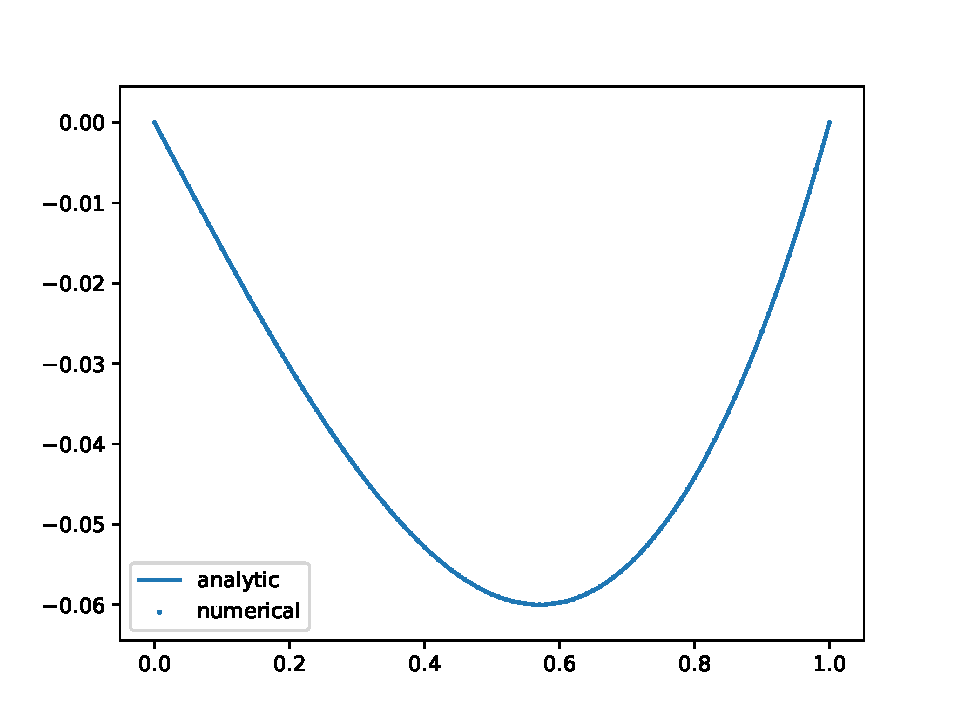
\includegraphics[width=0.75\textwidth]{code/relax.pdf}
    \caption{\label{fig:relax}}
\end{figure}

Running this you can see that theres are quite a few iteration needs to solve this equation. This can be accelerated by coarsening and then refining the grid in a technique known as multigrid. We won't cover this in this as in astrophysics there are other ways to solve this equation (FFTs for instance).

\subsection{Parabolic Problems}

As stated above, the parabolic problem has properties of both the hyperbolic and elliptic problem.  In particular, we will see that it can have very large propagation speeds like the elliptic problem, but can be solve in a flux-conservative way as in the hyperbolic problem.  Lets start with a prototypical problem
\be
\ddt{\Phi} = \dddx{\Phi}\label{eq:diffusion}
\ee
An identification of the flux to the $F = -\partial\Phi/\partial x$ allows us to write this like the flux-conservative equation
\be
\ddt{\Phi} + \ddx{F} = 0
\ee
If we presume the analytic ansatz
\be
\Phi(t,x) = \frac{\exp{-x^2/4t}}{t^{1/2}} + \Phi_0,
\ee
we see that it solve the diffusion equation (\ref{eq:diffusion}).  Lets try to solve this problem numerically.  Lets use a standard centered expression for the second derivative in Space
\be
\frac{\Phi^{n+1}_i - \Phi^n_i}{\Delta t} = \frac{\Phi^n_{i+1} - 2\Phi^n_i + \Phi^n_{i-1}}{\Delta x^2}
\ee
We can examine its stability in space with a single Fourier mode $\Phi_i^n = A^n\exp(-i2\pi x_i/L)$.  This gives
\be
\left|\frac{A^{n+1}}{A^n}\right| = \left|1 + 2\frac{\Delta t}{\Delta x^2}\left(\cos(2\pi\Delta x/L)-1\right)\right| < 1
\ee
which implies that $\Delta t \propto \Delta x^2/2$, e.g., the equivalent ``Courant'' number is $\alpha_{\rm CFL} = 2\Delta t/\Delta x^2$  So the timestep rapidly comes down as $\Delta x$ (higher resolution) shrinks.  

We can numerically solve this once we specific the boundary conditions over a finite domain.  However, we will note that the analytic solution spreads from $x=(-\infty,\infty)$.  However, if we put the boundaries far enough away, it will not ``pollute'' the solution too much in the region of interest.  Here the fact that the timescale goes like $t\sim L^2$ helps. 

Now lets examine the code in detail:

\lstinputlisting[language=Python]{code/parabolic.py}






%\newpage
%\section{Statistical Methods}

We will discuss statistical methods here.  Generally, statistical methods underly questions about statistical inference which is the ability to draw conclusions from data.  There are generally three questions that we may seek to answer:
\begin{enumerate}
  \item Parameter Estimation: What is the best estimate for a parameter, $\theta$, given some data.
  \item Confidence Estimation: How confident should be be in our parameter estimation.
  \item Hypothesis testing: How consistent is a given hypothesis with the available data.
\end{enumerate}
A few of you in astronomy and physics deal with this all the time.  A few more of you deal with this as part of your job as a TA or lecturer, after all, what is a grade but a estimate of the amount of student acquired knowledge/skills. 

In this context there are two paradigms, the classical or frequentist view and the Bayesian view.  In short, the classical view is based on 
\begin{enumerate}
  \item Probabilities are related to the relative frequency of events in the world. 
  \item Parameters are fixed constants -- they don't fluctuate.
  \item All things converge in the long-run.  A 95\% confidence interval means that over the long term, the measure parameter should fall within the 95\% confidence interval, 95\% of the time.
\end{enumerate}

On the other hand, the Bayesian view is based on.
\begin{enumerate}
  \item Probability describes the degree of subjective belief -- so parameters and models can have probabilities associated with them.
  \item Inference is done by looking at the probability distribution.  Probability distributions quantify the limits of our knowledge.
\end{enumerate}

So the battle between these two paradigms can be though of as a battle between confidence and distributions.  Because distributions are functions and are more difficult to calculate, Bayesian statistics are beset by large computational requirements, something is a familiar to some of you. 

\subsection{Maximum Likelihood}

The first things we will discuss is maximum likelihood estimation.  For that we need to come up with a likelihood function:
\be
L = p(D|M(\theta))
\ee
where $L$ is the likelihood, $D$ is the data and $M(\theta)$ is a models with parameters $\theta$.  A good likelihood estimator is a Gaussian estimator:
\be
p(D|M(\theta)) = \prod_{\rm data} \frac {1}{\sqrt{\pi\sigma_i}}\exp\left(-\left(\frac{x_i - \mu_i(\theta)}{\sigma_i}\right)^2\right)
\ee
Because of the nature of exponentials, it is easier to deal with the log likelihood which is 
\be
\log(L) = -\sum_{\rm data}\left(\frac{x_i - \mu_i(\theta)}{\sigma_i}\right)^2,
\ee
where we have thrown away an additive term which is constant in $\theta$.  

The log-likelihood is the function that we have to deal with when fitting functions to data.  Here we will take two examples.  In the first case, lets assume that we have a constant error $\sigma_i=\sigma$ and lets try to fit an polynomial to it. 

Now the polynomial is already baked into numpy as it is used all the time.  However, let's do something else.  We know that the underlying function is a sine function with noise, so lets fit a sine function to it. 

In doing so we will need to compute the error.  Here the error or residuals $r_i$ are the unsquared part of the likelihood function:
\be
r_i = \frac{x_i - \mu_i(\theta)}{\sigma_i}
\ee
Note that in this case that $r_i$ can be positive and negative.  

\subsection{$\chi^2$ statistic}

Sometimes we want to see how good a model fits the data.  In this case, we can define a $\chi^2$ statistic, which is 
\be
\chi^2 = \sum_{i=1}^N\left(\frac{x_i - \mu_i(\theta)}{\sigma_i}\right)^2
\ee
where $N$ denotes the number of data points.  Now $\chi^2$ get larger and larger as the number of data points increase.  So we need to define a ``normalized'' version of $\chi^2$, which is $\chi^2{\rm dof}$ of $\chi^2$ per degree of freedom.  For a model with p parameters and N data points the number of degrees of freedom is $N-p$. So
\be
\chi_{\rm dof}^2 = \frac{1}{N-k}\sum_{i=1}^N\left(\frac{x_i - \mu_i(\theta)}{\sigma_i}\right)^2
\ee
Now if the error is distributed normally, then for a good model $\chi_{\rm dof}$ is about unity.  Much larger and this means that model likely sucks given the error.  Much smaller might indicate the we don't understand our errors or their are overestimated.  Now generally, a order unity $\chi_{\rm dof}^2$ does not mean 

Go ahead and now compute the $\chi_{\rm dof}^2$.  Is it order unity?  You should find out that it is much smaller than unity.  What does this tell you?

\subsection{Markov-Chain Monte-Carlo}

Suppose you are given some distribution of the form $P$ and you want to compute the expectation value of y.  Then the formal term is 
\be
\left<y\right> = \int y dp
\ee
Or in other words 
\be
\left<y\right> = \int y P dV,
\ee
where $V$ represents some volume in phase (state) space and $P= dp/dV$ is the probability density function.  Now lets consider the case when the state space is descrete like in quantum mechanics 
\be
\left<y\right> = \frac{\sum_i y_i P(V_i)}{\sum_i P(V_i)},
\ee
where the denominator is just ensure that the sums are properly normalized.  To make this more concrete, lets consider the case where the state space is energy $V=E$ and $P$ follows a Maxwell-Boltzman distribution.  In this case we have
\be
\left<y\right> = \frac{\sum_i y_i \exp(-E_i/k_BT)}{\sum_i \exp(-E_i/k_BT)},
\ee
where you recognized the denominator as $Z = \sum_i \exp(-E_i/k_BT)$ is the partition function from statistical mechanics.  

Suppose now we want to do this sum using monte carlo methods.  Here we cannot sum over infinite number of states but over $N$ states so we have. 
\be
\left<y\right> = \frac{\sum_{i=1}^N y_i \exp(-E_i/k_BT)}{\sum_{i=1}^N \exp(-E_i/k_BT)},
\ee
The issue is that the space of $E_i$ is huge, but for most values of $E_i$, the contribution is small e.g. $\propto \exp(-E_i/k_BT)$.  So we want to pick random values of $E_i$ following a distribution that {\it maximizes the contribution to the sum}.  To do this let consider a expectation value over a weight function $w$
\be
\left<f\right>_w = \frac{\sum_j f_j w_j}{\sum_j w_j}
\ee
Now lets define the expectation value
\be
\left<\frac{yP(E)}{w}\right>_w = \frac{\sum_j y_j P(E_j) w_j/w_j}{\sum_j w_j} = \frac{\left<y\right> Z}{\sum_j w_j}
\ee
or in other words 
\be
\left<y\right> = \left<\frac{yP(E)}{w}\right>_w Z^{-1}\sum_j w_j
\ee
Now the trick is that I will pick $w = P(E)/Z$ so that I have (when I integrate monte carlo style) 
\be
\left<y\right> = N^{-1}\sum_{i=1}^N y_i
\ee
which is simply an average over my random points, but the difficulty is that I have to pick from a distribution that follows a PDF that is defined by the weight function $w = P(E)/Z$.  I do not necessarily know how to compute the partition function as it involves as integral over all phase space.  

At the point, we will use a Markov chain, which allows us to do this integral without exact knowledge of the complete PDF.  The way is works is as follows.  
\begin{enumerate}
    \item Starting a state i, make a small change to state j.
    \item compute the transition probability $\Delta P$
    \item draw a random number $r$ in $[0,1]$ and accept the move if $r<T_{ij}$; otherwise do nothing
\end{enumerate}
In the case of the weight function that follows a Maxwell-Boltzmann distribution, the transition probability can be computed from detailed balance where 
\be
 P(E_i)R_{ij} = P(E_j)R_{ji} \rightarrow  \Delta P = \frac{R_{ij}}{R_{ji}} = \frac{P(E_j)}{P(E_i)} = \exp\left(-\frac{\Delta E_{ij}}{k_BT}\right)
\ee
where $R_{ij}$ are the rates of going from the i-th state to the j-th state

To encode all this, let us introduce the Metropolis-Hasting algorithm.  
\begin{enumerate}
    \item Starting with some state $i$
    \item Generate a set of possible moves.
    \item Pick a random move $j$ from the generate set
    \item Accept the move with probability 
    \be
    P = \min\left(1,\exp(-\frac{\Delta E_{ij}}{k_BT}\right)
    \ee
\end{enumerate}

\subsection{Bayesian Statistics}

The biggest use of MCMC is its application to model fitting especially in the context of Bayesian modeling.  Usually in this case, we are concerned about the computation of the posterior distribution function $\pi(\vec{\theta};\vec{x})$ of parameters $\vec{\theta}$ given some data $\vec{x}$ and a prior $\pi(\vec{\theta})$.  We do this via Bayes' theorem
\be
\pi(\vec{\theta};\vec{x}) = \frac{\pi(\vec{\theta})p(\vec{x};\vec{\theta})}{p(\vec{x})}
\ee
where $p(\vec{x};\vec{\theta})$ is a likelihood function and $p(\vec{x}) = \int \pi(\vec{\theta})p(\vec{x};\vec{\theta})d\vec{\theta}$ is essentially the normalization. In essence, we want to compute
\be
p(\vec{x}) = \int \pi(\vec{\theta})p(\vec{x};\vec{\theta})d\vec{\theta}
\ee
The key is that we only want to compute over the values of $\theta$ that really contribute.  So we can define a Metropolis algorithm that goes for this as
\begin{enumerate}
    \item Begin with some parameter set $\vec{\theta}_1$ 
    \item Compute the joint likelihood $L_1 = \pi(\vec{\theta}_1)p(\vec{x};\vec{\theta}_1)$
    \item Pick a random proposal $\vec{\theta}_2$ from a distribution based on the priors.
    \item Compute the likelihood $L_2 = \pi(\vec{\theta}_2)p(\vec{x};\vec{\theta}_2)$
    \item Compute the transition probability $R = L_2/L_1$
    \item Accept the proposal with probability $R$
\end{enumerate}

Lets consider the computation of the expectation values of the parameters $\vec{\theta}$ over the distribution given by the posterior distribution, $\pi(\vec{\theta};\vec{x})$ or
\be
\left<\vec{\theta}\right>_{\pi} = \int \vec{\theta}\pi(\vec{\theta};\vec{x}) d\vec{\theta} 
\ee
If I compute this value, I get the expected value of the parameters.  If I plot out $\pi(\vec{\theta})$, I get the distribution of relevant $\theta$'s 

Thus I can use MCMC for this.  A subtle, but important point is that when I take the average over the entire Markov chain, then the values of the parameters should reduce to the expected value.  However, if I take the distribution of the parameters, i.e., take a histogram of the values of the parameters in the chain, the distribution of the parameters is the posterior distribution.  This is a subtle, but important point and in case you ever wondered how these parameters distributions for various models where ever generated, now you know. 

Lets solidify our understanding with a ``simple'' example.  Let us consider our noisy sin wave as before, which we reproduce for clarity

\begin{lstlisting}[language=Python]
def generate_data() :
    A = 5
    phi = np.pi/4
    sigma = 1.0
  
    theta = np.arange(-2*np.pi, 2*np.pi, 0.025*np.pi)
    y = A*np.sin(theta + phi) + np.random.normal(0, sigma, theta.size)
  
    return theta, y, np.array([A, phi])
\end{lstlisting}  

Now we will define a log-likelihood function
\be
\log p(\vec{y}; \vec{\theta}) = -\sum_i\left(\frac{y_i - \theta_0\sin(t_i + \theta_1)}{\sigma}\right)^2,
\ee
where we set $\sigma = 1$ and $t$ is an independent variable.  We need to set some priors. Lets set $\theta_0$ to be a flat distribution between 1 and 10 and $\theta_1$ to be a flat distribution between 0 and $2\pi$.  

\begin{lstlisting}[language=Python]
def priors( x) : 
    if(x[0] < 1 or x[0] > 10) : 
      return 0
    if(x[1] < 0 or x[1] > 2*np.pi) : 
      return 0
    return 1  
\end{lstlisting}

Here is the rest of the specification.  For your HW, you will implement the heart of the algorithm, move and the loglikelihood.

\begin{lstlisting}[language=Python]
def mcmc(func, t, y, x, burn_in=1000, MAX_CHAIN=500000) :
  xchain = [] 
  i = 0

  for j in range(MAX_CHAIN) : 
    x, accepted_move = move(func, t, y, x)
    if( accepted_move) :
      i += 1 
      if( i > burn_in) : 
        xchain.append(x)
  return np.array(xchain)

def move(func, t, y, x, h = 0.1, TINY=1e-30) :
    pass

def loglikelihood( func, t, y, x, sigma=1) : 
    pass

if __name__ == "__main__" : 
    t, y, x0 = generate_data()
    guess = np.zeros(2)
    guess[0] = 2
    guess[1] = 0
    xchain = mcmc(test_function, t, y, x0)
    print( "chain length = {2} MCMC mean = {0}, actual = {1}".format(str(np.average(xchain, axis=0)), str(x0), xchain.shape[0]))
    pl.hist2d(xchain[:,0],xchain[:,1],bins=100)
    pl.show()
    pl.clf()
    pl.hist(xchain[:,0],bins=100)
    pl.savefig("mcmc_1.pdf")

\end{lstlisting}

Note that we accumulate the values of $\vec{\theta}$ as we evolve the chain and we have burn in timescale of about 1000 moves.

Now, we can compute statistics using the distribution of parameters.  Go ahead and compute the 25th, 50th, and 75th percentile of the parameters using numpy.percentile.

%\lstinputlisting[language=Python]{code/mcmc.py}

%\begin{figure}
%    \centering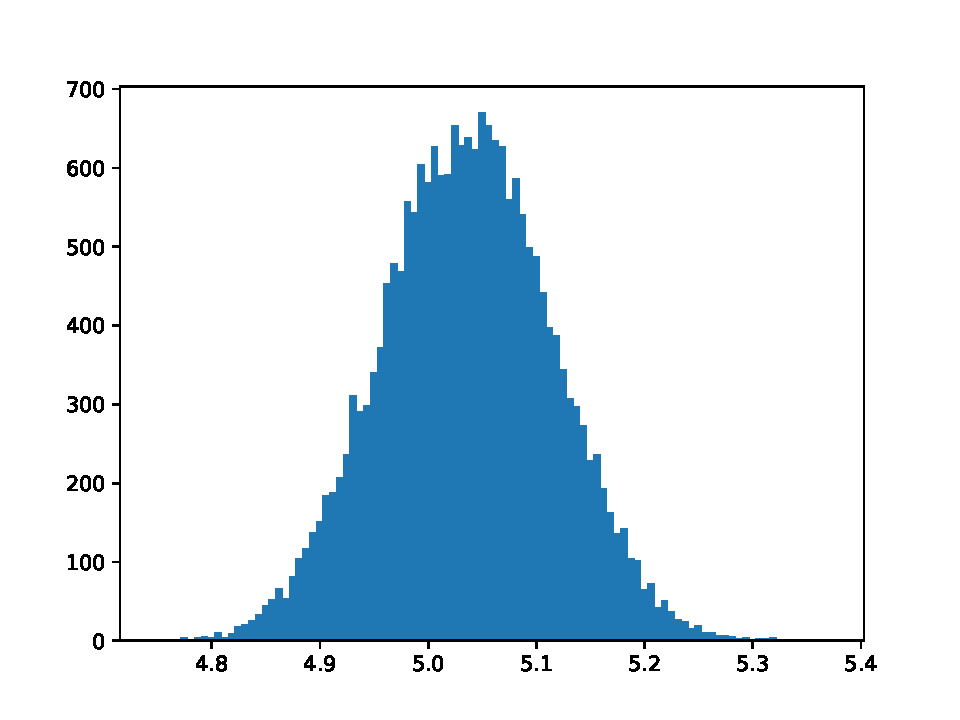
\includegraphics[width=0.75\textwidth]{code/mcmc_1.pdf}
%    \caption{\label{fig:mcmc}}
%\end{figure}

%\subsection{Simulated Annealing}





\end{document}
